\documentclass{article}
\usepackage[utf8]{inputenc}
\usepackage[colorlinks,linkcolor=black,urlcolor=blue]{hyperref}
\usepackage{color}
\usepackage{indentfirst}



\title{\textbf{Jadepix DAQ User Guide V0.1}}


%\author{ }
\date{January 2018}

\usepackage{natbib}
\usepackage{graphicx}

\begin{document}

\maketitle

\begin{table}[]
    \centering
    \begin{tabular}{c|c|c}
    \hline
        Version & Data & Comments \\
    \hline
        V0.1 & 1/18/2018 & Setup manual\\
    \hline
    \end{tabular}
\end{table}


\setcounter{page}{0}
\thispagestyle{empty}

\newpage

\tableofcontents
\setcounter{page}{0}
\thispagestyle{empty}

\newpage

\section{Introduction}
JadePixDAQ is the software package for managing the interface with JadePix sensors developed by the IHEP CMOS Collaboration. 

\section{Requirements}
The software runs on Windows machines parentally. It is under developing with Windows 7, so it is not stable.


\section{Basic Hardware}
    The basic system consists of:

    \begin{itemize}
        \item Computer with PCIE 
        \item KC705 Board
        \item MotherBoard
        \item Daughterboard
    \end{itemize}

\section{Software installation}

    \subsection{Address:}
        \url{https://github.com/cepc/kc705}
        
    \subsection{ Dependencies:}
        \begin{itemize}
            \item Swig: \url{http://swig.org/}
            \item CMake: \url{https://cmake.org/}
            \item Python: On  Windows, it is recommend to use Anaconda version
                
            \begin{itemize}
                \item \url{https://anaconda.org/anaconda/python}
                \item If you want to compile code with library from ROOT and convert to python, please download 32 bit Anaconda
                \item Fast mirror:\url{http://mirrors.ustc.edu.cn/anaconda/archive/}
            \end{itemize}
                
            \item Visual studio 2017 community: \\
            \url{https://www.visualstudio.com/downloads/}
            
        \end{itemize}

    \subsection{Compile:}
        \begin{itemize}
            \item Open cmake-gui:
            
                \begin{itemize}
                    \item o	If you want compile with ROOT, specify the generator to Visual Studio 15 2017 Win32, otherwise, you can install with Visual Studio 15 2017 Win64. Please make sure your python library is corresponding with the generator. You can see an example in the following.
                    
                    %%%%%%
                    \begin{figure}[h!]
                    \centering
                    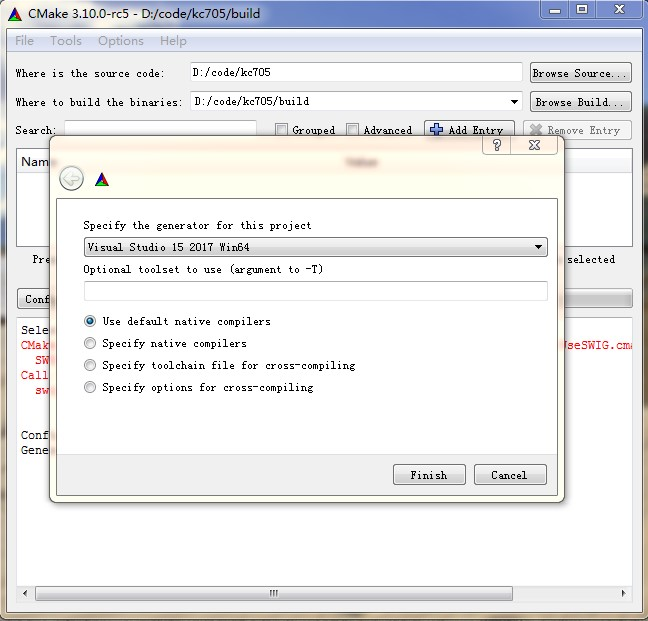
\includegraphics[scale=1.7,height=5cm]{Figures/Cmake_1.jpg}
                    %\caption{???}
                    %\label{fig:???}
                    \end{figure}
                    %%%%%%%
                    
                \end{itemize}
            
            \item Set environment:
            
                \begin{itemize}
                
                    \item Select the path of swig
                    \item Select the path of python
                    \item If you don’t want to select manually, you can set the system PATH:\\
                    {\color{cyan} Computer $\to$ Properties $\to$ Advanced system setting $\to$ Environment $\to$ Path (double click) $\to$ Add (use “;” to split)}
                    \item After finished:
                    
                        %%%%%%
                        \begin{figure}[h!]
                        \centering
                        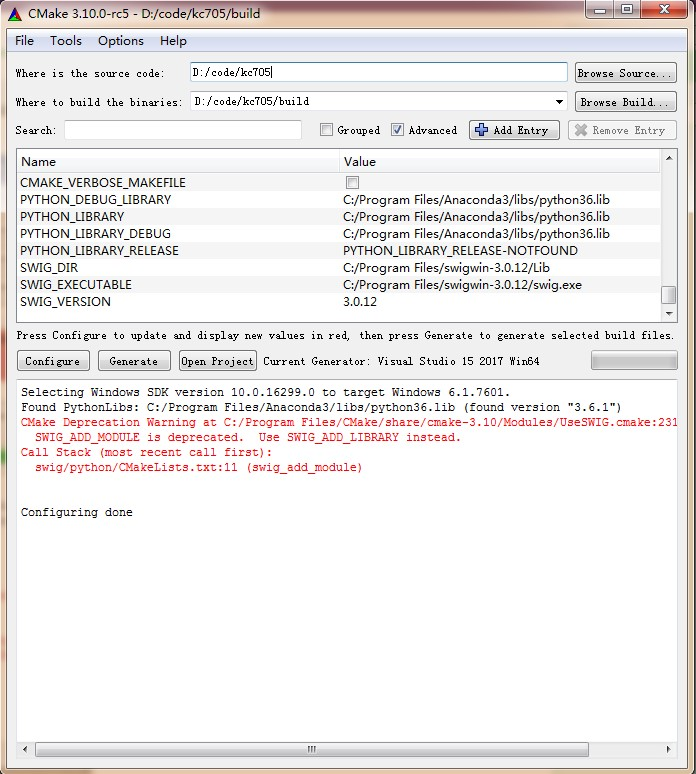
\includegraphics[scale=1.7,height=5cm]{Figures/Cmake_2.jpg}
                        %\caption{The Universe}
                        %\label{fig:univerise}
                        \end{figure}
                        %%%%%%%
                    
                
                \end{itemize}
            
            \item Configure $\to$ Generate $\to$ Open Project,then visual studio 2017 open with the project
                %%%%%%
                \begin{figure}[h!]
                \centering
                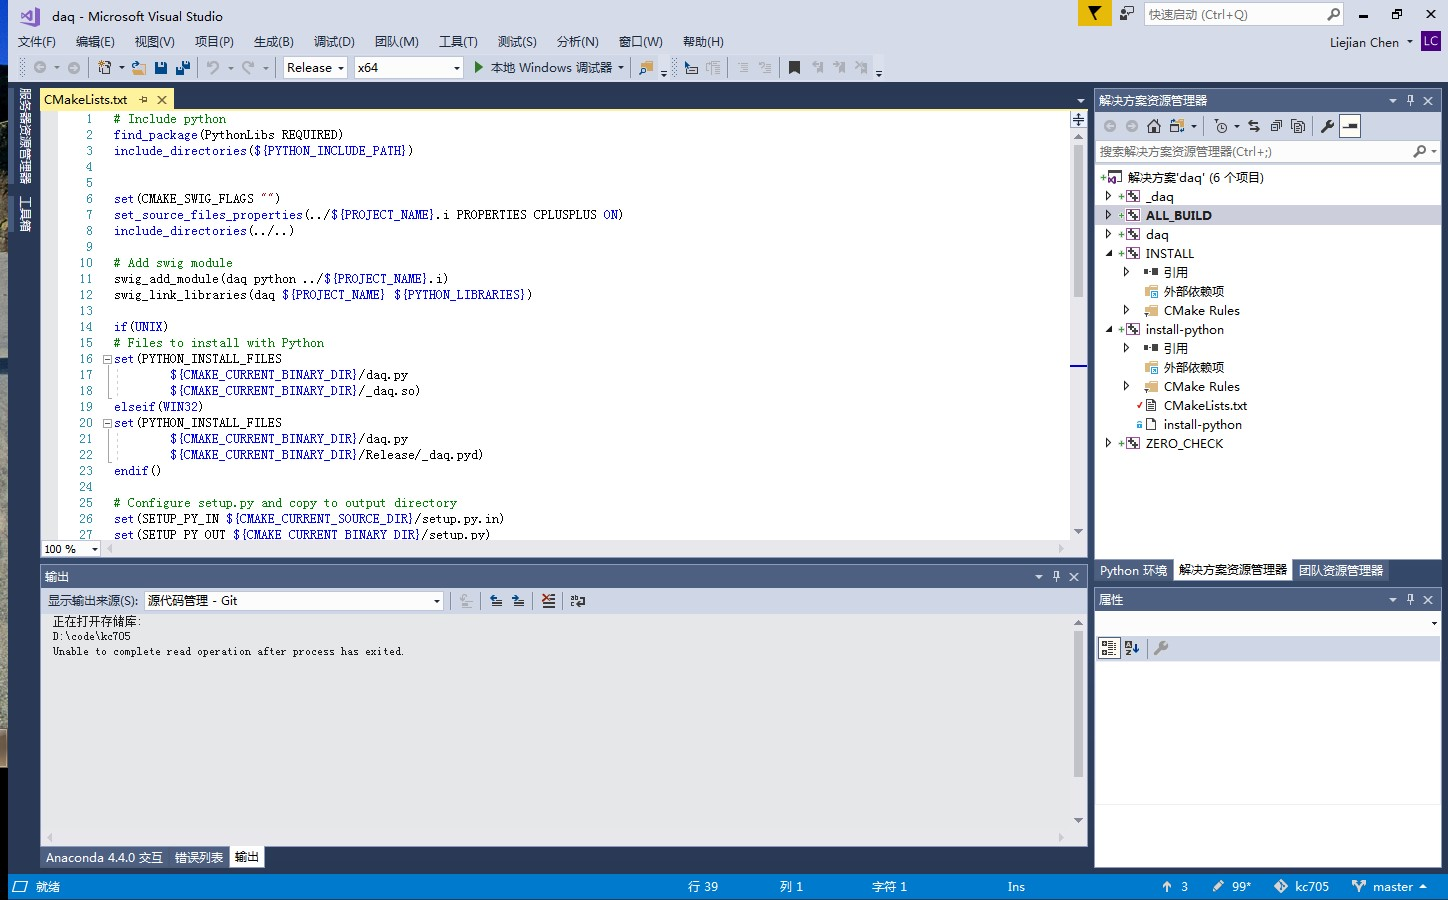
\includegraphics[scale=1.7,height=5cm]{Figures/VS_1.jpg}
                %\caption{The Universe}
                %\label{fig:univerise}
                \end{figure}
                %%%%%%%
                
                \begin{itemize}
                    \item Select Release to generate
                    \item Ignore the warning: it cannot open the program (We just generate the lib and python module)
                    
                        %%%%%%
                        \begin{figure}[h!]
                        \centering
                        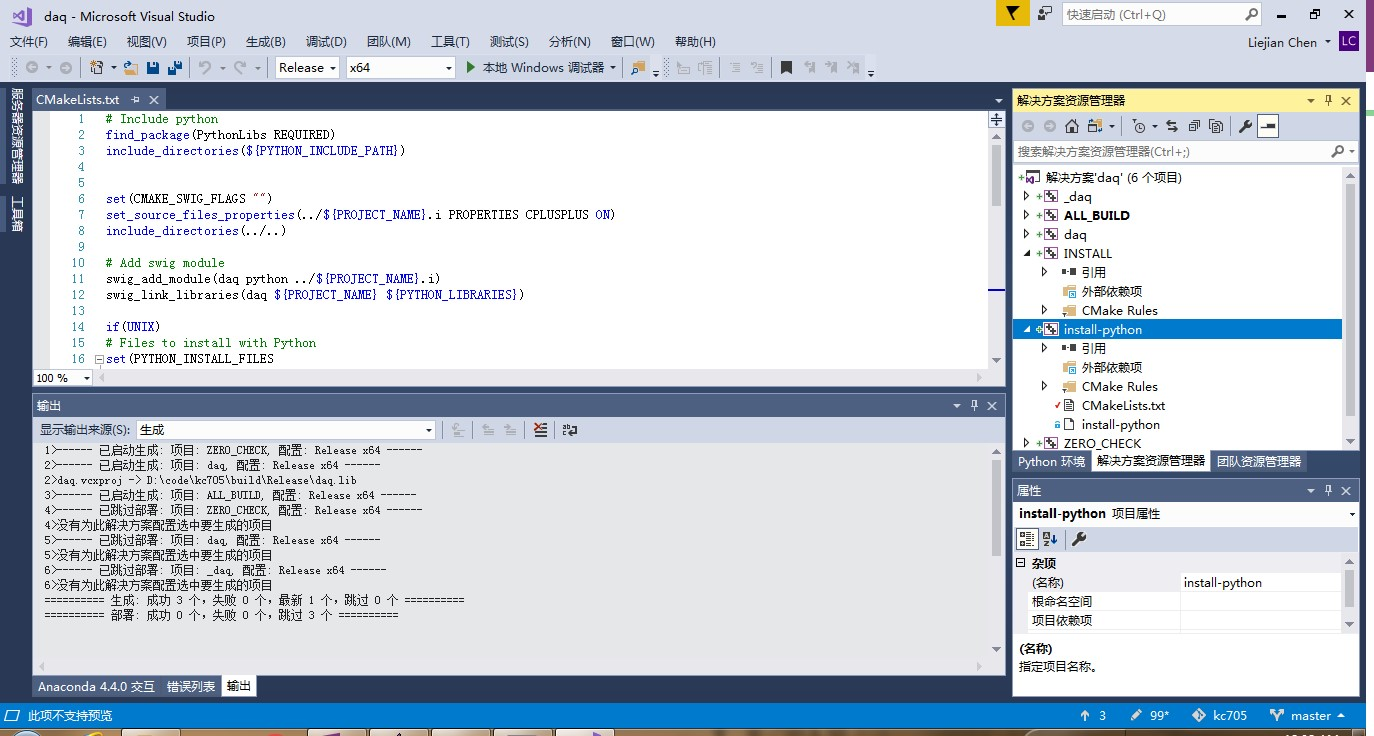
\includegraphics[scale=1.7,height=5cm]{Figures/VS_2.jpg}
                        %\caption{}
                        %\label{fig:}
                        \end{figure}
                        %%%%%%%
                    
                    \item Click the install python with right mouse button->Generate. If it failed, make sure you have the right permission
                    
                        %%%%%%
                        \begin{figure}[h!]
                        \centering
                        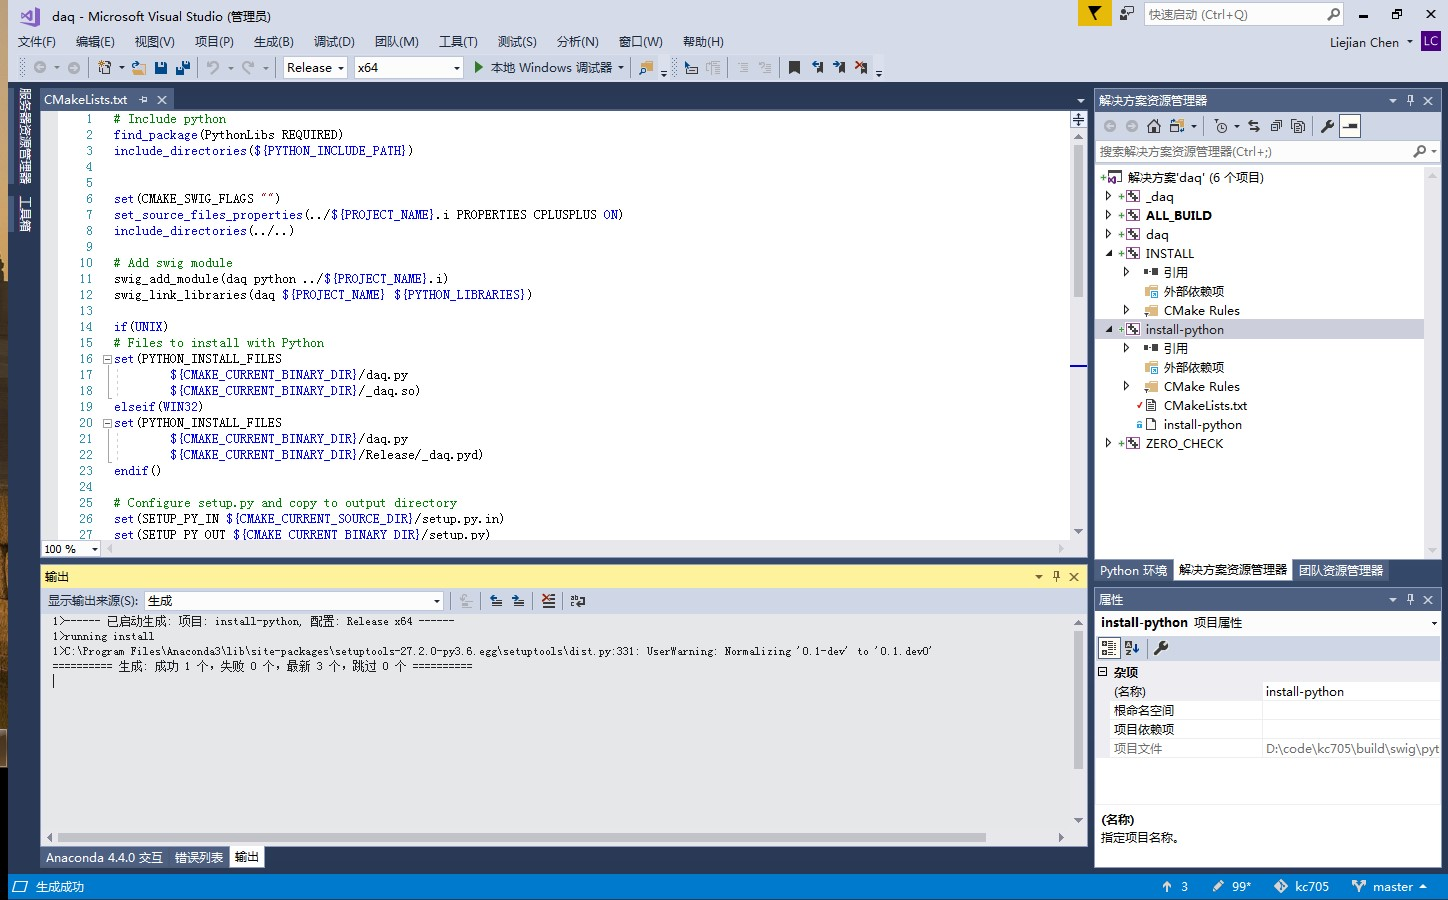
\includegraphics[scale=1.7,height=5cm]{Figures/VS_3.jpg}
                        %\caption{}
                        %\label{fig:}
                        \end{figure}
                        %%%%%%%
                        If it is successful, the python module daq is installed in your python lib site-packages.
                        
                    
                \end{itemize}
                
            \item Open it in your command terminal:
                \begin{itemize} 
                
                    \item Make sure your terminal has  python environment setting. 
                    \item If not, click Computer $\to$ Properties $\to$ Advanced system setting $\to$ Environment $\to$ path $\to$ ADD python path
                    
                        %%%%%%
                        \begin{figure}[h!]
                        \centering
                        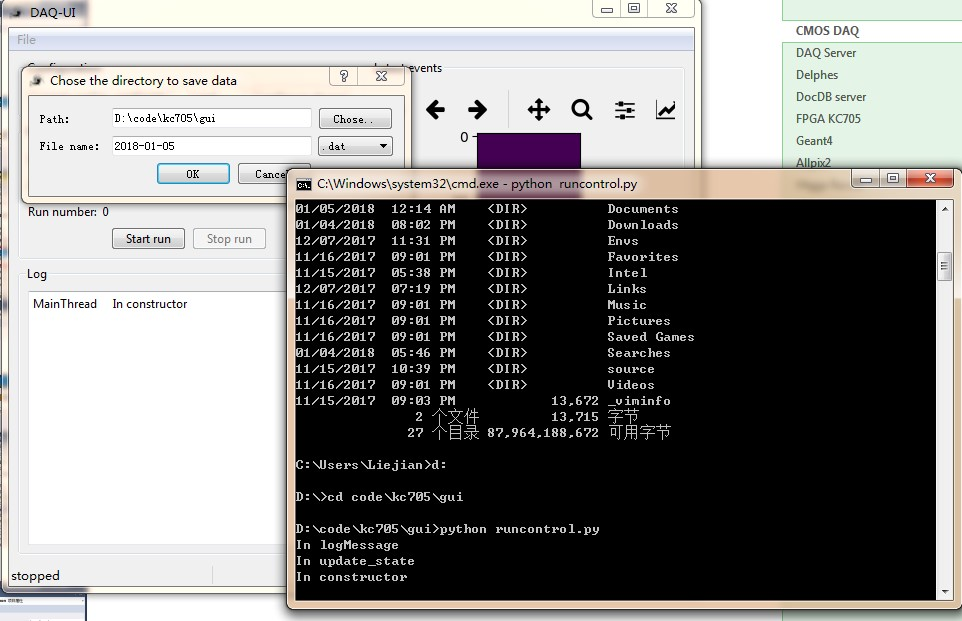
\includegraphics[scale=1.7,height=5cm]{Figures/Open.jpg}
                        %\caption{}
                        %\label{fig:}
                        \end{figure}
                        %%%%%%%
                    
                    
                \end{itemize}
                
            
            
        \end{itemize}
    
\section{Software status:}
   %%%%%%
    \begin{figure}[h!]
    \centering
    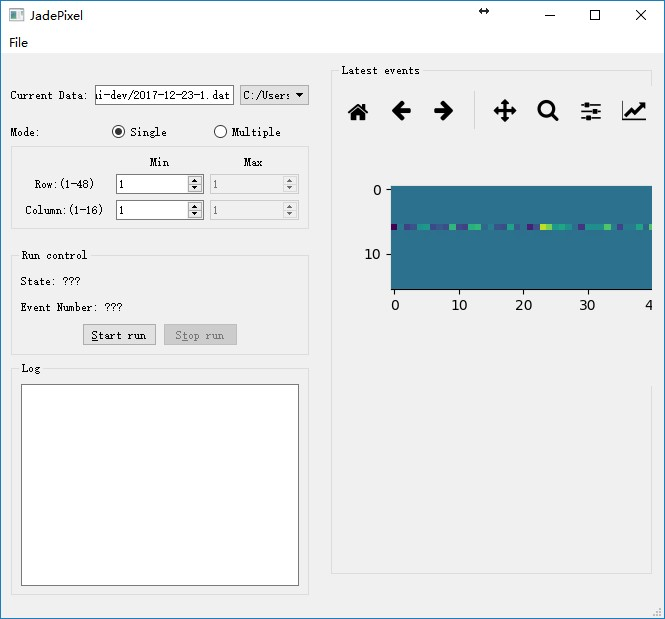
\includegraphics[scale=1.7,height=5cm]{Figures/GUI.jpg}
    %\caption{}
    %\label{}
    \end{figure}
    %%%%%%%
     
    \begin{itemize}
     
        \item Online data taking: not real test
        \item Offline data analysis: primary test
        \item Row/Column select: GUI finish without API from FPGA
        \item Log: More important information need be added
        \item Display: hit map, need a fast pedestal/ADC spectrum view
        \item Decode: slow but can work
         
    \end{itemize}

%\newpage



\section{Software development}

    \subsection{ File structure:}
    
    KC705:
            
        \begin{itemize}
            
            \item analysis: Ryuta’s code to decode and analysis raw data
            \item doc: documents and notes
            \item exe: generator binary execute program, CONSIDER DELETE
            \item fpga: firmware develop source files using Vivado
            \item gui: online GUI and related python code
            \item include: daq head file
            \item onlineAnalysis: reference Ryuta’s code but remove ROOT . It is used for online display
            \item src: daq src file
            \item swig: python blinding
            \item test: some sample data
            \item xillybus: FPGA program
            \item CMakeList: compile tool macro
            \item README.md: general guide 
            \item build\_env.bat: On Windows, the useful  environment setting.
            \item build\_env.sh: Useful environment setting for UNIX/LINUX
            \item build\_env\_mingw.bat: MingGW 64 setting, CONSIDER DELETE
            \item build\_swig.bat: auto script to compile with Make (Visual studio)
                
        \end{itemize}
        
    \subsection{A primary plan:}
        
        \begin{itemize}
            
            \item Task
                
                \begin{itemize}
                    
                    \item Cleanup: 22 Jan
                    \item Configuration:
                        
                        \begin{itemize}
                            
                            \item Row/Col select: 5 Jan
                            \item Multiple file save:  29 Jan
                                
                        \end{itemize}
                            
                    \item Online analysis:
                        
                        \begin{itemize} 
                            
                            \item Online monitor, hit map: 29 Jan
                            \item fast pedestal/ADC spectrum: 5 Jan
                                
                        \end{itemize}
                            
                    \item Offline fast analysis: When  a run of data just finish, apply fast analysis with GUI: 29 Jan
                    \item Platform: change to LINUX  April
                    \item Related to test beam: TO ADD 
                        
                \end{itemize}
                
                
        \end{itemize}
        
        
    
%\newpage



\section{Contributors}

    \begin{itemize}
    
        \item \textbf{Xin: Manager}
        \item Jason
        \item Liejian
        \item Xiaoxu
        \item Ryuta
        \item Kai
        \item Tao
        \item Yi
        ...
        
    \end{itemize}

\end{document}
